\documentclass{report}

\usepackage{fullpage}
\usepackage[skip=4pt]{caption} % ``skip'' sets the spacing between the figure and the caption.
\usepackage{pgfplots}   % Needed for plotting
\usepackage{amsmath}    % Allows for piecewise functions using the ``cases'' construct
\usepackage{graphics}
\usepackage{grffile}   % Allows period in the graphics file name

\usepackage[obeyspaces,spaces]{url} % Used for typesetting with the ``path'' command
\usepackage[hidelinks]{hyperref}   % Make the cross references clickable hyperlinks

%\renewcommand\thesection{\arabic{section}} % Prevent chapter number in section number.

\newcommand{\eref}[1]{(\ref{#1})}
\newcommand{\includeLambdaPlot}[1]{  
\begin{figure}
    \includegraphics[width=1.0\textwidth]{img/test_train_compare_d=19_lambda=#1.pdf}
    \caption{Comparison of Test Data and Predicted Output with Training $\lambda$=#1}
\end{figure}}

\renewcommand{\baselinestretch}{2}
\author{Andrew Stolman \& \\Zayd Hammoudeh}
\title{CMPS242 HW01 \textendash {} Polynomial Learning}
\begin{document}
  \maketitle
  
  \begin{figure}
    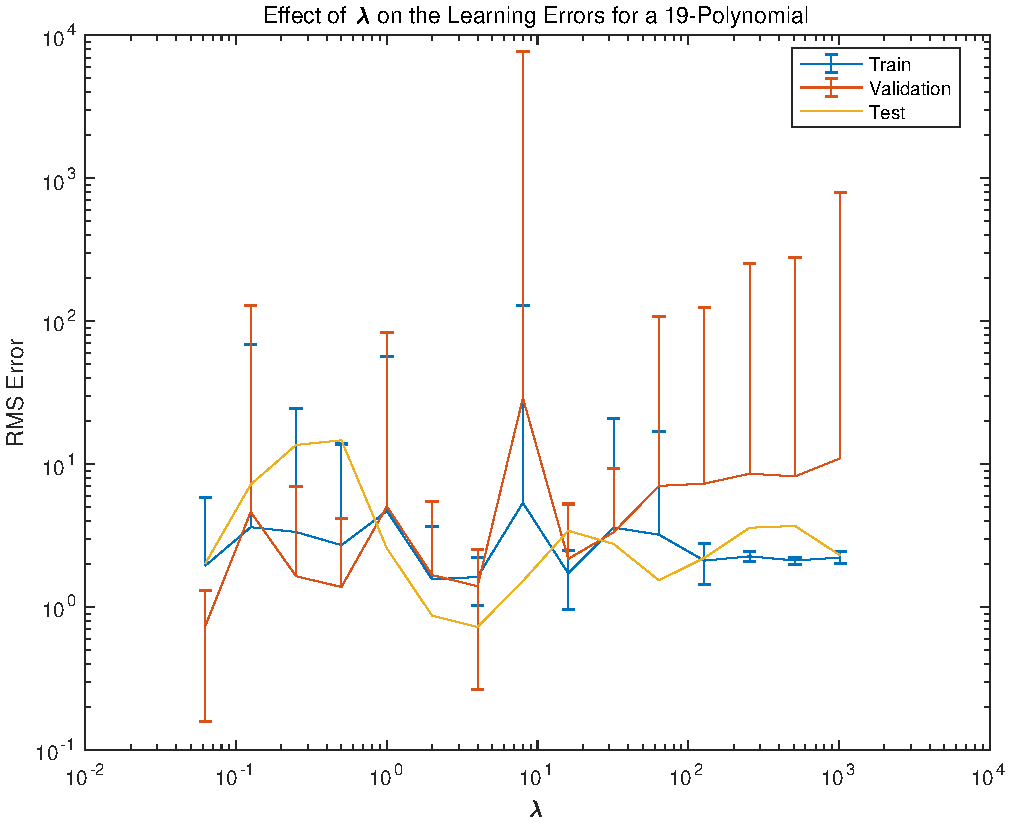
\includegraphics[width=1.0\textwidth]{img/lambda_sweep_degree=19.pdf}
    \caption{Effect of $\lambda$ on the Training, Validation, and Test Errors}
  \end{figure}

  \includeLambdaPlot{0.00}
  \includeLambdaPlot{0.06}
  \includeLambdaPlot{0.12}
  \includeLambdaPlot{0.25}
  \includeLambdaPlot{0.50}
  \includeLambdaPlot{1.00}
  \includeLambdaPlot{2.00}
  \includeLambdaPlot{4.00}
  \includeLambdaPlot{8.00}
  \includeLambdaPlot{16.00}
  \includeLambdaPlot{32.00}
  \includeLambdaPlot{64.00}
  \includeLambdaPlot{128.00}
  \includeLambdaPlot{256.00}
  \includeLambdaPlot{512.00}
  \includeLambdaPlot{1024.00}

\end{document}